% Template of basic phisics experiment 基于 article template,在此基础上做修改
% 设定文章编码类型,正文字号为五号则 zihao=5,正文字号为小四则 zihao=-4
\documentclass[zihao=5, UTF8]{article}		


% 自定义宏定义
\def\N{\mathbb{N}}
\def\F{\mathbb{F}}
\def\Z{\mathbb{Z}}
\def\Q{\mathbb{Q}}
\def\R{\mathbb{R}}
\def\C{\mathbb{C}}
\def\T{\mathbb{T}}
\def\S{\mathbb{S}}
\def\A{\mathbb{A}}
\def\I{\mathscr{I}}
\def\d{\mathrm{d}}
\def\p{\partial}


% 物理实验报告所需的其它宏包
\usepackage{ulem}   % \uline 下划线支持

% 导入基本宏包
\usepackage[UTF8]{ctex}     % 设置文档为中文语言
\usepackage[colorlinks, linkcolor=blue, anchorcolor=blue, citecolor=blue, urlcolor=blue]{hyperref}  % 宏包:自动生成超链接 (此宏包与标题中的数学环境冲突)
% \usepackage{docmute}    % 宏包:子文件导入时自动去除导言区,用于主/子文件的写作方式,\include{./51单片机笔记}即可。注:启用此宏包会导致.tex文件capacity受限。
\usepackage{amsmath}    % 宏包:数学公式
\usepackage{mathrsfs}   % 宏包:提供更多数学符号
\usepackage{amssymb}    % 宏包:提供更多数学符号
\usepackage{pifont}     % 宏包:提供了特殊符号和字体
\usepackage{extarrows}  % 宏包:更多箭头符号

% 列表环境设置
\usepackage{enumitem}   % 宏包:列表环境设置
    \setlist[enumerate]{itemsep=0pt, parsep=0pt, topsep=0pt, partopsep=0pt, leftmargin=3.5em} 
    \setlist[itemize]{itemsep=0pt, parsep=0pt, topsep=0pt, partopsep=0pt, leftmargin=3.5em}
    \newlist{circledenum}{enumerate}{1} % 创建一个新的枚举环境  
    \setlist[circledenum,1]{  
        label=\protect\circled{\arabic*}, % 使用 \arabic* 来获取当前枚举计数器的值,并用 \circled 包装它  
        ref=\arabic*, % 如果需要引用列表项,这将决定引用格式(这里仍然使用数字)
        itemsep=0pt, parsep=0pt, topsep=0pt, partopsep=0pt, leftmargin=3.5em
    }  
% 文章页面 margin 设置
\usepackage[a4paper]{geometry}  % 宏包:文章页面 margin 设置
    \geometry{top=0.75in}
    \geometry{bottom=0.75in}
    \geometry{left=0.75in}
    \geometry{right=0.75in}   % 设置上下左右页边距
    \geometry{marginparwidth=1.75cm}    % 设置边注距离(注释、标记等)

% 自定义数学环境
\usepackage{amsthm} % 宏包:数学环境配置
% theorem-line 环境自定义
    \newtheoremstyle{MyLineTheoremStyle}% <name>
        {11pt}% <space above>
        {11pt}% <space below>
        {}% <body font> 使用默认正文字体
        {}% <indent amount>
        {\bfseries}% <theorem head font> 设置标题项为加粗
        {:}% <punctuation after theorem head>
        {.5em}% <space after theorem head>
        {\textbf{#1}\thmnumber{#2}\ \ (\,\textbf{#3}\,)}% 设置标题内容顺序
    \theoremstyle{MyLineTheoremStyle} % 应用自定义的定理样式
    \newtheorem{LineTheorem}{Theorem.\,}
% theorem-block 环境自定义
    \newtheoremstyle{MyBlockTheoremStyle}% <name>
        {11pt}% <space above>
        {11pt}% <space below>
        {}% <body font> 使用默认正文字体
        {}% <indent amount>
        {\bfseries}% <theorem head font> 设置标题项为加粗
        {:\\ \indent}% <punctuation after theorem head>
        {.5em}% <space after theorem head>
        {\textbf{#1}\thmnumber{#2}\ \ (\,\textbf{#3}\,)}% 设置标题内容顺序
    \theoremstyle{MyBlockTheoremStyle} % 应用自定义的定理样式
    \newtheorem{BlockTheorem}[LineTheorem]{Theorem.\,} % 使用 LineTheorem 的计数器
% definition 环境自定义
    \newtheoremstyle{MySubsubsectionStyle}% <name>
        {11pt}% <space above>
        {11pt}% <space below>
        {}% <body font> 使用默认正文字体
        {}% <indent amount>
        {\bfseries}% <theorem head font> 设置标题项为加粗
        {:\\ \indent}% <punctuation after theorem head>
        {0pt}% <space after theorem head>
        {\textbf{#3}}% 设置标题内容顺序
    \theoremstyle{MySubsubsectionStyle} % 应用自定义的定理样式
    \newtheorem{definition}{}


% 有色文本框及其设置
\usepackage[dvipsnames,svgnames]{xcolor}    %设置插入的文本框颜色
\usepackage[strict]{changepage}     % 提供一个 adjustwidth 环境
\usepackage{framed}     % 实现方框效果
    \definecolor{graybox_color}{rgb}{0.95,0.95,0.96} % 文本框颜色。修改此行中的 rgb 数值即可改变方框纹颜色,具体颜色的rgb数值可以在网站https://colordrop.io/ 中获得。(截止目前的尝试还没有成功过,感觉单位不一样)(找到喜欢的颜色,点击下方的小眼睛,找到rgb值,复制修改即可)
    \newenvironment{graybox}{%
    \def\FrameCommand{%
    \hspace{1pt}%
    {\color{gray}\small \vrule width 2pt}%
    {\color{graybox_color}\vrule width 4pt}%
    \colorbox{graybox_color}%
    }%
    \MakeFramed{\advance\hsize-\width\FrameRestore}%
    \noindent\hspace{-4.55pt}% disable indenting first paragraph
    \begin{adjustwidth}{}{7pt}%
    \vspace{2pt}\vspace{2pt}%
    }
    {%
    \vspace{2pt}\end{adjustwidth}\endMakeFramed%
    }

% 各级标题自定义设置
\usepackage{titlesec}   
    % section标题自定义设置 
    \titleformat{\section}[hang]{\normalfont\huge\bfseries\centering}{第\,\thesection\,部分}{20pt}{}
    % subsection标题自定义设置 
    \titleformat{\subsection}[hang]{\normalfont\Large\bfseries}{\,\thesubsection\,}{8pt}{}
    % subsubsection标题自定义设置
    \titleformat{\subsubsection}[hang]{\normalfont\large\bfseries}{\,\thesubsubsection\,}{6pt}{}

% 外源代码插入设置
\usepackage{matlab-prettifier}
    \lstset{
        style=Matlab-editor,  % 继承matlab代码颜色等
    }
\usepackage[most]{tcolorbox} % 引入tcolorbox包 
\usepackage{listings} % 引入listings包
    \tcbuselibrary{listings, skins, breakable}
    \lstdefinestyle{matlabstyle}{
        language=Matlab,
        basicstyle=\small,
        breakatwhitespace=false,
        breaklines=true,
        captionpos=b,
        keepspaces=true,
        numbers=left,
        numbersep=15pt,
        showspaces=false,
        showstringspaces=false,
        showtabs=false,
        tabsize=2
    }
    \newtcblisting{matlablisting}{
        arc=0pt,
        top=0pt,
        bottom=0pt,
        left=1mm,
        listing only,
        listing style=matlabstyle,
        breakable,
        colback=white   % 选一个合适的颜色
    }
    % 自定义Verilog代码样式
\lstdefinelanguage{Verilog}{
    keywords=[1]{module, input, output, wire, assign, endmodule},
    keywords=[2]{always, if, else, case, endcase, begin, end},
    sensitive=true,
    morecomment=[l]{//},
    morecomment=[s]{/*}{*/},
    morestring=[b]",
}

\lstset{
    language=Verilog,
    basicstyle=\ttfamily\small,
    keywordstyle=[1]\color{blue},
    keywordstyle=[2]\color{purple},
    commentstyle=\color{gray},
    stringstyle=\color{orange},
    showstringspaces=false,
    numbers=left,
    numberstyle=\tiny\color{gray},
    stepnumber=1,
    numbersep=5pt,
    frame=single,
    tabsize=4,
    breaklines=true,
    backgroundcolor=\color{lightgray!10}
}

% table 支持
\usepackage{booktabs}   % 宏包:三线表
\usepackage{tabularray} % 宏包:表格排版
\usepackage{longtable}  % 宏包:长表格
\usepackage{tabularx}  % 宏包:宽表格
\usepackage{multirow}  % 宏包:表格中一格显示多个项目
\usepackage{tikz}   % 宏包:绘图
\usetikzlibrary{automata, positioning}  % TikZ绘图库

% figure 设置
\usepackage{graphicx}  % 支持 jpg, png, eps, pdf 图片 
\usepackage{svg}       % 支持 svg 图片
    \svgsetup{
        % 指向 inkscape.exe 的路径
        inkscapeexe = C:/aa_MySame/inkscape/bin/inkscape.exe, 
        % 一定程度上修复导入后图片文字溢出几何图形的问题
        inkscapelatex = false                 
    }


% 图表进阶设置
\usepackage{float}     % 图表位置浮动设置 
\usepackage{caption}    % 图注、表注
    \captionsetup[figure]{name=图}  
    \captionsetup[table]{name=表}
    \captionsetup{labelfont=bf, font=small}

% 文章默认字体设置
    \usepackage{fontspec}   % 宏包:字体设置
       \setmainfont{SimSun}    % 设置中文字体为宋体字体
      \setCJKmainfont[AutoFakeBold=3]{SimSun} % 设置加粗字体为 SimSun 族,AutoFakeBold 可以调整字体粗细^     \setmainfont{Times New Roman} % 设置英文字体为Times New Roman

% 代码环境设置
\usepackage{minted}


% 其它设置
    % equation 公式编号设置
        \makeatletter  
        \renewcommand{\theequation}{\thesection.\arabic{equation}}  
        \makeatother
    % 脚注设置
        \renewcommand\thefootnote{\ding{\numexpr171+\value{footnote}}}
    % 参考文献引用设置
        \bibliographystyle{unsrt}   % 设置参考文献引用格式为unsrt
        \newcommand{\upcite}[1]{\textsuperscript{\cite{#1}}}     % 自定义上角标式引用
    % 文章序言设置
        \newcommand{\cnabstractname}{序言}
        \newenvironment{cnabstract}{%
            \par\Large
            \noindent\mbox{}\hfill{\bfseries \cnabstractname}\hfill\mbox{}\par
            \vskip 2.5ex
            }{\par\vskip 2.5ex}


% 页眉页脚设置
\usepackage{fancyhdr}   %宏包:页眉页脚设置
    \pagestyle{fancy}
    \fancyhf{}
    \cfoot{\thepage}
    \renewcommand\headrulewidth{1pt}
    \renewcommand\footrulewidth{0pt}
    %\rhead{\bfseries 分组序号: YK04-2}    
    \chead{《数字电路》实验报告,\ 韩初晓,\ 2023K8009908002}
    \lhead{2024.11.19}

% 文档信息设置
%\title{这里是标题\\The Title of the Report}
%\author{丁毅\\ \footnotesize 中国科学院大学,北京 100049\\ Yi Ding \\ %\footnotesize University of Chinese Academy of Sciences, Beijing %100049, China}
%\date{\footnotesize 2024.8 -- 2025.1}

% 开始编辑文章

\begin{document}
%\noindent\begin{flushright}
%   \zihao{2}{分组序号: YK04-2}
%\end{flushright}

\setCJKfamilyfont{boldsong}[AutoFakeBold = {2.17}]{SimSun}
\newcommand*{\boldsong}{\CJKfamily{boldsong}}


\begin{center}\large
    \noindent{\Huge\bfseries\boldsong《数字电路》实验报告 }
    \\\vspace{0.4cm}
    \noindent\textit{
        \textbf{\boldsong 实验名称:}\uline{\hspace{1.7cm} 状态机实验\hspace{1.7cm}}\hspace{0.4cm} 
        指导教师:\uline{\hspace{1.0cm}王珎,范志华\hspace{1.0cm}}}
    \\\vspace{0.1cm}
    \noindent\textit{
        姓名:\uline{\,\,\,韩初晓\,\,\,}\hspace{0.2cm}
        学号:\uline{\,\,\,{\upshape 2023K8009908002}\,\,\,}\hspace{0.2cm}
        专业:\uline{\,\,\,计算机科学与技术\,\,\,}\hspace{0.2cm}
        班级:\uline{\,\,\,\upshape{2306}\,\,\,}}
    \\\vspace{0.1cm}
    \noindent\textit{
        实验日期:\uline{\,\,{\upshape 2024.10.17}\,\,}\hspace{0.2cm}
        实验地点:\uline{\,\,\,教学楼{\upshape224}\,\,\,}\hspace{0.2cm}
        是否调课/补课:\uline{\hspace{0.5cm}否\hspace{0.5cm}}\hspace{0.2cm}
        成绩:\uline{\hspace{2cm}}}
\end{center}
% \vspace{-0.2cm}
\noindent\rule{\textwidth}{0.1em}   % 分割线

% 控制目录不换页
\vspace{1cm}
\setcounter{tocdepth}{2}  % 目录深度为 2(不显示 subsubsection)
\noindent\begin{minipage}{\textwidth}\centering
\tableofcontents\thispagestyle{fancy}   % 显示页码、页眉等   
\end{minipage}  
\newpage

\section{实验目的}\thispagestyle{fancy}
\begin{enumerate}
    \item 熟悉verilog 编程、调试。
    \item 熟悉状态机的工作原理,能熟练编写状态机程序。
\end{enumerate}

\section{实验环境}
\begin{itemize}
    \item Vivado 2017.4 开发工具
    \item FPGA 开发平台(根据手册中的默认设置进行选择)
\end{itemize}


\section{实验内容}


\subsection{实验一:读取0110的有限状态自动机}  
\subsubsection{原理说明}  
本实验实现了一个具有五个状态的同步状态机,接受 \texttt{0110} 为合法输入。模块根据输入信号 \texttt{in} 和当前状态 \texttt{state},决定下一状态 \texttt{next\_state} 并输出状态相关信号 \texttt{out}。有限状态机的具体状态及其行为如下:  
\begin{itemize}  
    \item \textbf{S0}:初始状态,当输入信号 \texttt{in} 为 0 时,转移到状态 S1;否则保持在 S0。  
    \item \textbf{S1}:当 \texttt{in} 为 1 时,转移到状态 S2;否则保持在 S1。  
    \item \textbf{S2}:当 \texttt{in} 为 1 时,转移到状态 S3;否则返回到状态 S1。  
    \item \textbf{S3}:当 \texttt{in} 为 1 时,转移回状态 S0;否则转移到状态 S4。  
    \item \textbf{S4}:当 \texttt{in} 为 1 时,返回状态 S2;否则返回状态 S1。  
\end{itemize}  

状态转换图如下所示:  

\begin{center}
  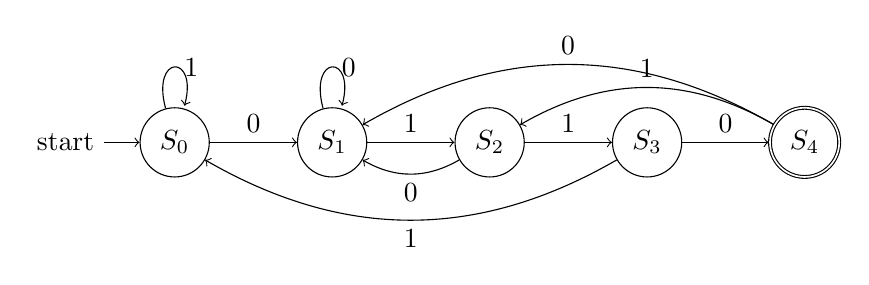
\begin{tikzpicture}[node distance=2cm]
    \node[state, initial] (S0) {$S_0$};
    \node[state, right of=S0] (S1) {$S_1$};
    \node[state, right of=S1] (S2) {$S_2$};
    \node[state, right of=S2] (S3) {$S_3$};
    \node[state, right of=S3, accepting] (S4) {$S_4$};

    % Transitions
    \draw[->] (S0) edge node[above] {0} (S1);
    \draw[->] (S1) edge node[above] {1} (S2);
    \draw[->] (S2) edge node[above] {1} (S3);
    \draw[->] (S3) edge node[above] {0} (S4);

    \draw[->] (S0) edge [loop above] node[right] {1} (S0);
    \draw[->] (S1) edge [loop above] node[right] {0} (S1);
    \draw[->] (S4) edge [bend right] node[above] {0} (S1);
    \draw[->] (S3) edge [bend left] node[below] {1} (S0);
    \draw[->] (S4) edge [bend right] node[above] {1} (S2);
    \draw[->] (S2) edge [bend left] node[below] {0} (S1);
  \end{tikzpicture}
\end{center}

输出信号 \texttt{out} 在状态 S4 时为高电平(1),其他状态下为低电平(0)。模块的状态转移逻辑由时钟信号 \texttt{clk} 和复位信号 \texttt{rstn} 控制。  

\subsubsection{接口定义}  
\begin{itemize}  
    \item 输入信号:  
    \begin{itemize}  
        \item \texttt{clk}:时钟信号,用于同步状态转移。  
        \item \texttt{rstn}:异步复位信号,低电平有效,复位时状态返回至初始状态 S0。  
        \item \texttt{in}:输入控制信号,决定状态转移路径。  
    \end{itemize}  
    \item 输出信号:  
    \begin{itemize}  
        \item \texttt{out}:状态机的输出信号,当状态为 S4 时为高电平(1),其他状态为低电平(0)。  
    \end{itemize}  
\end{itemize}  

\subsubsection{调试过程及结果}  
通过编写 \texttt{fsm\_1} 模块的 Testbench,对其状态转移行为进行了仿真测试。测试时,输入信号 \texttt{in} 在不同状态下进行了切换,并验证了模块的状态转移与输出行为。仿真波形如下所示:  
\begin{figure}[htbp]  
    \centering  
    \includegraphics[width=\textwidth]{fsm_1.png} % 图片路径和大小  
    \caption{\texttt{fsm\_1} 模块的仿真测试结果}  
    \label{fig:fsm_1_simulation}  
\end{figure}  

通过观察仿真波形可以验证:  
\begin{itemize}  
    \item 在复位信号 \texttt{rstn} 低电平时,状态机正确返回初始状态 S0。  
    \item 状态机在每个状态下均按照设计逻辑正确转移。  
    \item 输出信号 \texttt{out} 在状态 S4 时为高电平,表明读取到了合法信号 \texttt{0110} ,状态机的功能符合预期设计。  
\end{itemize}  



\subsection{实验二:读取1011的有限状态自动机}  
\subsubsection{原理说明}  
本实验实现了一个有限状态机(FSM),用于根据输入信号 \texttt{in} 的变化生成特定的输出信号 \texttt{out} ,接受 \texttt{1011} 为合法输入。有限状态机包含五个状态,通过输入信号和当前状态确定下一状态,并在特定状态下产生输出信号。状态的具体定义及其行为如下:  
\begin{itemize}  
    \item \textbf{S0}:初始状态,当 \texttt{in} 为 1 时,转移到状态 S1;否则保持在 S0。  
    \item \textbf{S1}:当 \texttt{in} 为 0 时,转移到状态 S2;否则保持在 S1。  
    \item \textbf{S2}:当 \texttt{in} 为 1 时,转移到状态 S3;否则返回到状态 S0。  
    \item \textbf{S3}:当 \texttt{in} 为 1 时,转移到状态 S4;否则转移到状态 S2。  
    \item \textbf{S4}:当 \texttt{in} 为 1 时,返回状态 S1;否则转移到状态 S2。  
\end{itemize}  

状态转换图如下所示:  

\begin{center}
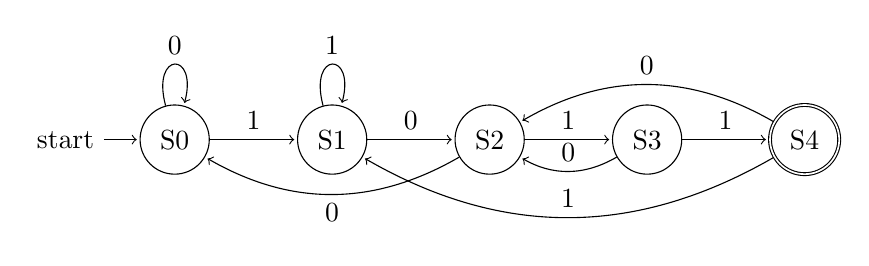
\begin{tikzpicture}[shorten >=1pt, node distance=2cm, on grid, auto]
   % 定义状态节点
   \node[state, initial] (s0) {S0};
   \node[state] (s1) [right=of s0] {S1};
   \node[state] (s2) [right=of s1] {S2};
   \node[state] (s3) [right=of s2] {S3};
   \node[state, accepting] (s4) [right=of s3] {S4};

   % 绘制状态转移
   \path[->]
   % S0 的转移
   (s0) edge [loop above] node {0} (s0)
        edge [above] node {1} (s1)
   % S1 的转移
   (s1) edge [above] node {0} (s2)
        edge [loop above] node {1} (s1)
   % S2 的转移
   (s2) edge [above] node {1} (s3)
        edge [bend left, below] node {0} (s0)
   % S3 的转移
   (s3) edge [above] node {1} (s4)
        edge [bend left, above] node {0} (s2)
   % S4 的转移
   (s4) edge [bend left, above] node {1} (s1)
        edge [bend right, above] node {0} (s2);
\end{tikzpicture}
\end{center}

输出信号 \texttt{out} 在状态 S4 时为高电平(1),表明读取到了 \texttt{1011} 的合法输入信号,其他状态为低电平(0)。状态机由时钟信号 \texttt{clk} 驱动,并在复位信号 \texttt{rstn} 低电平时回到初始状态 S0。  

\subsubsection{接口定义}  
\begin{itemize}  
    \item 输入信号:  
    \begin{itemize}  
        \item \texttt{clk}:时钟信号,用于同步状态转移。  
        \item \texttt{rstn}:异步复位信号,低电平有效,复位时状态返回至初始状态 S0。  
        \item \texttt{in}:输入信号,决定状态转移路径。  
    \end{itemize}  
    \item 输出信号:  
    \begin{itemize}  
        \item \texttt{out}:输出信号,在状态 S4 时为高电平(1),其余状态为低电平(0)。  
    \end{itemize}  
\end{itemize}  

\subsubsection{调试过程及结果}  
通过编写 \texttt{fsm\_2} 模块的 Testbench,对其状态转移和输出信号的生成逻辑进行了仿真测试。在仿真中,通过设置不同的输入信号 \texttt{in},验证了状态转移路径及输出信号是否符合设计要求。仿真波形如下所示:  
\begin{figure}[htbp]  
    \centering  
    \includegraphics[width=\textwidth]{fsm_2.png} % 图片路径和大小  
    \caption{\texttt{fsm\_2} 模块的仿真测试结果}  
    \label{fig:fsm_2_simulation}  
\end{figure}  

从仿真结果中可以验证:  
\begin{itemize}  
    \item 状态机在复位信号 \texttt{rstn} 为低电平时,正确返回初始状态 S0。  
    \item 状态机在不同输入条件下正确完成状态转移。  
    \item 输出信号 \texttt{out} 仅在状态 S4 时为高电平,表明读取到了 \texttt{1011} 的合法输入信号,符合设计要求。  
\end{itemize}  


\subsection{实验三:实现信号生成器模块}  
\subsubsection{原理说明}  
该信号生成器模块实现了一个具有12个状态的有限状态机(FSM),通过输入信号 \texttt{clk} 和复位信号 \texttt{rstn} 来控制状态转移,并根据当前状态生成输出信号 \texttt{out}。信号生成器的状态及其行为如下:  
\begin{itemize}  
    \item \textbf{S0}:初始状态,输出信号 \texttt{out} 为 0,转移到状态 S1。  
    \item \textbf{S1}:输出信号 \texttt{out} 为 0,转移到状态 S2。  
    \item \textbf{S2}:输出信号 \texttt{out} 为 1,转移到状态 S3。  
    \item \textbf{S3}:输出信号 \texttt{out} 为 0,转移到状态 S4。  
    \item \textbf{S4}:输出信号 \texttt{out} 为 1,转移到状态 S5。  
    \item \textbf{S5}:输出信号 \texttt{out} 为 0,转移到状态 S6。  
    \item \textbf{S6}:输出信号 \texttt{out} 为 0,转移到状态 S7。  
    \item \textbf{S7}:输出信号 \texttt{out} 为 1,转移到状态 S8。  
    \item \textbf{S8}:输出信号 \texttt{out} 为 1,转移到状态 S9。  
    \item \textbf{S9}:输出信号 \texttt{out} 为 0,转移到状态 S10。  
    \item \textbf{S10}:输出信号 \texttt{out} 为 1,转移到状态 S11。  
    \item \textbf{S11}:输出信号 \texttt{out} 为 1,转移回状态 S0。  
\end{itemize}  

状态机通过时钟信号 \texttt{clk} 进行同步操作,并在复位信号 \texttt{rstn} 低电平时返回初始状态 S0。  

\subsubsection{接口定义}  
\begin{itemize}  
    \item 输入信号:  
    \begin{itemize}  
        \item \texttt{clk}:时钟信号,用于同步状态转移。  
        \item \texttt{rstn}:异步复位信号,低电平有效,复位时状态返回至初始状态 S0。  
    \end{itemize}  
    \item 输出信号:  
    \begin{itemize}  
        \item \texttt{out}:输出信号,依据当前状态生成对应的输出。  
    \end{itemize}  
\end{itemize}  

\subsubsection{调试过程及结果}  
通过编写 \texttt{signal\_generator} 模块的 Testbench,对其状态转移和输出信号的生成进行了仿真测试。测试时,输入信号 \texttt{clk} 周期性变化,复位信号 \texttt{rstn} 用于初始化,验证了状态机在不同状态下的转移情况及输出信号的正确性。仿真波形如下所示:  
\begin{figure}[htbp]  
    \centering  
    \includegraphics[width=\textwidth]{signal_generator.png} % 图片路径和大小  
    \caption{\texttt{signal\_generator} 模块的仿真测试结果}  
    \label{fig:signal_generator_simulation}  
\end{figure}  

从仿真结果中可以验证:  
\begin{itemize}  
    \item 状态机在复位信号 \texttt{rstn} 为低电平时,正确返回初始状态 S0。  
    \item 状态机在不同输入信号作用下,能够正确完成状态转移,周期性输出 \texttt{001010011011}。  
\end{itemize}  

\subsection{实验四:自动报纸贩卖机}  
\subsubsection{原理说明}  
实验中实现了自动报纸贩卖机模块,它接受 1 分、2 分和 5 分硬币,并根据投入的硬币金额判断是否发放报纸。每当用户投入总额达到 5 分时,系统会发放报纸。  

该有限状态机共有 6 个状态,每个状态表示售货机的不同金额累计情况,描述如下:  
\begin{itemize}  
    \item \textbf{S0}:初始状态,未收到任何硬币。  
    \item \textbf{S1}:收到 1 分硬币,总金额为 1 分。  
    \item \textbf{S2}:收到 2 分硬币,总金额为 2 分。  
    \item \textbf{S3}:收到 3 分硬币,总金额为 3 分。  
    \item \textbf{S4}:收到 4 分硬币,总金额为 4 分。  
    \item \textbf{S5}:收到 5 分硬币,总金额为 5 分,发放报纸。  
\end{itemize}  

状态机的状态转换图如下所示:

\begin{center}
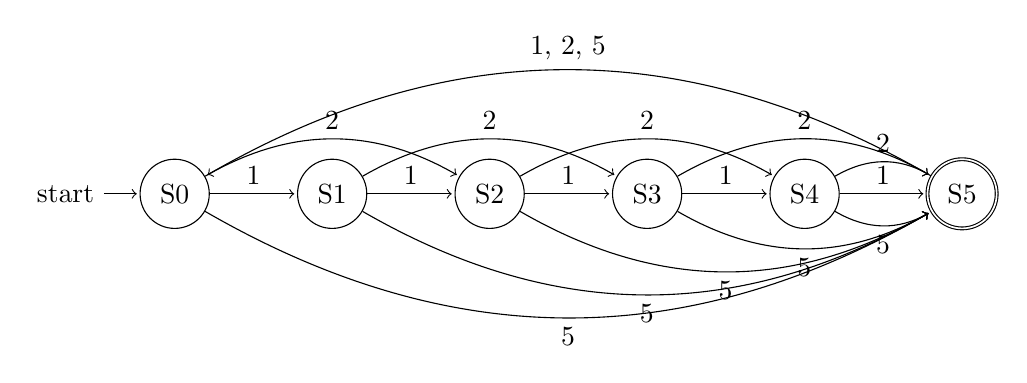
\begin{tikzpicture}[shorten >=1pt, node distance=2cm, on grid, auto]
   % 定义状态节点
   \node[state, initial] (s0) {S0};
   \node[state] (s1) [right=of s0] {S1};
   \node[state] (s2) [right=of s1] {S2};
   \node[state] (s3) [right=of s2] {S3};
   \node[state] (s4) [right=of s3] {S4};
   \node[state, accepting] (s5) [right=of s4] {S5};

   % 绘制转移箭头
   \path[->]
   % 从 S0 出发
   (s0) edge [above] node {1} (s1)
        edge [bend left, above] node {2} (s2)
        edge [bend right, below] node {5} (s5)
   % 从 S1 出发
   (s1) edge [above] node {1} (s2)
        edge [bend left, above] node {2} (s3)
        edge [bend right, below] node {5} (s5)
   % 从 S2 出发
   (s2) edge [above] node {1} (s3)
        edge [bend left, above] node {2} (s4)
        edge [bend right, below] node {5} (s5)
   % 从 S3 出发
   (s3) edge [above] node {1} (s4)
        edge [bend left, above] node {2} (s5)
        edge [bend right, below] node {5} (s5)
   % 从 S4 出发
   (s4) edge [above] node {1} (s5)
        edge [bend left, above] node {2} (s5)
        edge [bend right, below] node {5} (s5)
   % 从 S5 自环
   (s5) edge [bend right, above] node {1, 2, 5} (s0);
\end{tikzpicture}
\end{center}

每次投入硬币时,模块会根据硬币的面值调整状态,直到累计金额达到 5 分为止。如果投入的金额已满足 5 分,输出信号 \texttt{dispense} 为 1,表示发放报纸。

\subsubsection{接口定义}  
\begin{itemize}  
    \item 输入信号:  
    \begin{itemize}  
        \item \texttt{clk}:时钟信号,用于同步状态转移。  
        \item \texttt{rstn}:异步复位信号,低电平有效,复位时状态返回至初始状态 S0。  
        \item \texttt{coin[2:0]}:输入的硬币面值,支持三种硬币:  
        \begin{itemize}  
            \item 1 分硬币对应 3'b001  
            \item 2 分硬币对应 3'b010  
            \item 5 分硬币对应 3'b100  
        \end{itemize}  
    \end{itemize}  
    \item 输出信号:  
    \begin{itemize}  
        \item \texttt{dispense}:输出信号,当总金额达到 5 分时为高电平(1),表示发放报纸;否则为低电平(0)。  
    \end{itemize}  
\end{itemize}  

\subsubsection{调试过程及结果}  
通过编写 \texttt{newspaper\_machine} 模块的 Testbench,对其状态转移和发放报纸逻辑进行了仿真测试。在测试过程中,输入不同面额的硬币并观察状态变化和输出信号 \texttt{dispense} 的变化。仿真结果如下所示:  
\begin{figure}[htbp]  
    \centering  
    \includegraphics[width=\textwidth]{newspaper_machine.png} % 图片路径和大小  
    \caption{\texttt{newspaper\_machine} 模块的仿真测试结果}  
    \label{fig:newspaper_machine_simulation}  
\end{figure}  

从仿真结果中可以验证:  
\begin{itemize}  
    \item 状态机能够正确识别投入的硬币(1 分、2 分或 5 分),并进行正确的状态转移。  
    \item 当总金额达到 5 分时,输出信号 \texttt{dispense} 正确地变为高电平,表示报纸已发放。  
    \item 如果硬币不足以达到 5 分,状态机会根据硬币继续增加总金额,而不会发放报纸。  
\end{itemize}  


\section{实验总结}

在本实验中,我实现了四个有限状态自动机模块,深入体会了在verilog中设计时序电路的方法。在过度实验中,我了解了一段式、两段式和三段式自动机的设计,发现三段式状态机分为状态转移快,状态获取块和结果输出块三部分的代码结构更加清晰,也更加易于设计。本实验涉及到的有限状态自动机均为Moore型状态机,即状态机的输出仅与当前状态有关,而不依赖于输入信号。这代表着结果输出块可以通过将\texttt{state}作为敏感信号来实现。同时,在状态转移块中非阻塞赋值的应用也是本实验中的重要内容,在这一部分使用非阻塞赋值时需要规定信号的上升沿和下降沿。但是,在状态获取块中则需要使用阻塞赋值,这是特别需要注意的一点。在编写Testbench的时候,我注意到,对于检测输入序列是否合法的有限状态自动机,输入 \texttt{in} 信号的变化频率应当与模块中定义的时钟翻转频率相同,否则会造成错误。总的来说,本次实验让我对有限状态自动机的设计有了更深入的了解,也提高了我对verilog编程的熟练程度。

\section{源代码}

\subsection{实验一:读取0110的有限状态自动机}

\subsubsection{fsm\_1 模块源代码}

\begin{lstlisting}[language=Verilog]

module fsm_1(
    input clk,
    input rstn,
    input in,
    output reg out
    );
    
    localparam S0 = 3'b000;
    localparam S1 = 3'b001;
    localparam S2 = 3'b010;
    localparam S3 = 3'b011;
    localparam S4 = 3'b100;

    reg [2:0] state, next_state;

    always @(posedge clk or negedge rstn) begin
      if (~rstn) begin
          state <= S0;
      end
      else begin
          state <= next_state;
      end
    end

    always @(state or in) begin
      case(state)
        S0: begin
          if(in) begin
            next_state = S0;
          end
          else begin
            next_state = S1;
          end
        end
        S1: begin
          if(in) begin
            next_state = S2;
          end
          else begin
            next_state = S1;
          end
        end
        S2: begin
          if(in) begin
            next_state = S3;
          end
          else begin
            next_state = S1;
          end
        end
        S3: begin
          if(in) begin
            next_state = S0;
          end
          else begin
            next_state = S4;
          end
        end
        S4: begin
          if(in) begin
            next_state = S2;
          end
          else begin
            next_state = S1;
          end
        end
        default: next_state = S0;
      endcase
    end

    always @(state) begin
      case(state)
        S0:out = 1'b0;
        S1:out = 1'b0;
        S2:out = 1'b0;
        S3:out = 1'b0;
        S4:out = 1'b1;
        default: out = 1'b0;
      endcase
    end
endmodule

\end{lstlisting}

\subsubsection{fsm\_1 模块 Testbench}

\begin{lstlisting}[language=Verilog]
module test_fsm_1(
    );
    reg clk;
    reg rstn;
    reg in;
    wire out;

    fsm_1 instance_fsm_1(
      .clk(clk),
      .rstn(rstn),
      .in(in),
      .out(out)
      );

    initial begin
      clk = 0;
      rstn = 1;
      #0.1 rstn = 0;
      #1.1 rstn = 1;
    end

    initial begin
      in = 0;
      #1 in = 0;
      #1 in = 1;
      #1 in = 1;
      #1 in = 0;
      #1 in = 1;
      #1 in = 0;
      #1 in = 0;
    end

    always begin
      #1 in = $random() % 2;
    end

    always begin
      #0.5 clk = ~clk;
    end
endmodule
\end{lstlisting}

\subsection{实验二:读取1011的有限状态自动机}

\subsubsection{fsm\_2 模块源代码}

\begin{lstlisting}[language=Verilog]

module fsm_2(
    input clk,
    input rstn,
    input in,
    output reg out
    );
    
    localparam S0 = 3'b000;
    localparam S1 = 3'b001;
    localparam S2 = 3'b010;
    localparam S3 = 3'b011;
    localparam S4 = 3'b100;

    reg [2:0] state, next_state;

    always @(posedge clk or negedge rstn) begin
      if (~rstn) begin
          state <= S0;
      end
      else begin
          state <= next_state;
      end
    end

    always @(state or in) begin
      case(state)
        S0: begin
          if(in) begin
            next_state = S1;
          end
          else begin
            next_state = S0;
          end
        end
        S1: begin
          if(in) begin
            next_state = S1;
          end
          else begin
            next_state = S2;
          end
        end
        S2: begin
          if(in) begin
            next_state = S3;
          end
          else begin
            next_state = S0;
          end
        end
        S3: begin
          if(in) begin
            next_state = S4;
          end
          else begin
            next_state = S2;
          end
        end
        S4: begin
          if(in) begin
            next_state = S1;
          end
          else begin
            next_state = S2;
          end
        end
        default: next_state = S0;
      endcase
    end

    always @(state) begin
      case(state)
        S0:out = 1'b0;
        S1:out = 1'b0;
        S2:out = 1'b0;
        S3:out = 1'b0;
        S4:out = 1'b1;
        default: out = 1'b0;
      endcase
    end
endmodule

\end{lstlisting}

\subsubsection{fsm\_2 模块 Testbench}

\begin{lstlisting}[language=Verilog]
module test_fsm_2(
    );
    reg clk;
    reg rstn;
    reg in;
    wire out;

    fsm_2 instance_fsm_2(
      .clk(clk),
      .rstn(rstn),
      .in(in),
      .out(out)
      );

    initial begin
      clk = 0;
      rstn = 1;
      #0.1 rstn = 0;
      #1.1 rstn = 1;
    end

    initial begin
      in = 0;
      #1 in = 1;
      #1 in = 0;
      #1 in = 1;
      #1 in = 1;
      #1 in = 0;
      #1 in = 1;
      #1 in = 1;
      #1 in = 0;
      #1 in = 1;
      #1 in = 0;
      #1 in = 0;
      #1 in = 1;
      #1 in = 0;
    end

    always begin
      #1 in = $random() % 2;
    end

    always begin
      #0.5 clk = ~clk;
    end
endmodule

\end{lstlisting}

\subsection{实验三:实现信号生成器模块}

\subsubsection{signal\_generator 模块源代码}

\begin{lstlisting}[language=Verilog]

module signal_generator(
    input clk,
    input rstn,
    output reg out
    );

    localparam S0 = 4'b0000;
    localparam S1 = 4'b0001;
    localparam S2 = 4'b0010;
    localparam S3 = 4'b0011;
    localparam S4 = 4'b0100;
    localparam S5 = 4'b0101;
    localparam S6 = 4'b0110;
    localparam S7 = 4'b0111;
    localparam S8 = 4'b1000;
    localparam S9 = 4'b1001;
    localparam S10 = 4'b1010;
    localparam S11 = 4'b1011;

    reg [3:0] state, next_state;

    always @(posedge clk or negedge rstn) begin
      if (~rstn) begin
        state <= S0;
      end
      else begin
        state <= next_state;
      end
    end

    always @(state) begin
      case(state)
        S0: begin
          next_state = S1;
          out = 1'b0;
        end
        S1: begin
          next_state = S2;
          out = 1'b0;
        end
        S2: begin
          next_state = S3;
          out = 1'b1;
        end
        S3: begin
          next_state = S4;
          out = 1'b0;
        end
        S4: begin
          next_state = S5;
          out = 1'b1;
        end
        S5: begin
          next_state = S6;
          out = 1'b0;
        end
        S6: begin
          next_state = S7;
          out = 1'b0;
        end
        S7: begin
          next_state = S8;
          out = 1'b1;
        end
        S8: begin
          next_state = S9;
          out = 1'b1;
        end
        S9: begin
          next_state = S10;
          out = 1'b0;
        end
        S10: begin
          next_state = S11;
          out = 1'b1;
        end
        S11: begin
          next_state = S0;
          out = 1'b1;
        end
        endcase
    end
endmodule

\end{lstlisting}

\subsubsection{signal\_generator 模块 Testbench}

\begin{lstlisting}[language=Verilog]
module test_signal_generator(

    );
    reg clk;
    reg rstn;
    wire out;

    signal_generator instance_signal_generator(
      .clk(clk),
      .rstn(rstn),
      .out(out)
      );

    initial begin
      clk = 0;
      rstn = 1;
      #0.1 rstn = 0;
      #0.1 rstn = 1;
    end

    always begin
      #0.5 clk = ~clk;
    end
endmodule
\end{lstlisting}

\subsection{实验四:实现自动报纸贩卖机}

\subsubsection{newspaper\_machine 模块源代码}

\begin{lstlisting}[language=Verilog]

module newspaper_machine(
    input clk,
    input rstn,
    input [2:0] coin,
    output reg dispense
    );

    reg [2:0] state, next_state;
    localparam S0 = 3'b000;
    localparam S1 = 3'b001;
    localparam S2 = 3'b010;
    localparam S3 = 3'b011;
    localparam S4 = 3'b100;
    localparam S5 = 3'b101;

    always @(posedge clk or negedge rstn) begin
      if (~rstn) begin
        state <= S0;
      end else begin
        state <= next_state;
      end
    end

    always @(coin or state) begin
      case (state)
      S0: begin
        if (coin == 3'b001) begin
          next_state = S1;
        end 
        else if (coin == 3'b010) begin
          next_state = S2;
        end 
        else if (coin == 3'b101) begin
          next_state = S5;
        end
        else begin
          next_state = S0;
        end
      end
      S1: begin
        if (coin == 3'b001) begin
          next_state = S2;
        end
        else if (coin == 3'b010) begin
          next_state = S3;
        end
        else if (coin == 3'b101) begin
          next_state = S5;
        end
        else begin
          next_state = S1;
        end
      end
      S2: begin
        if (coin == 3'b001) begin
          next_state = S3;
        end 
        else if (coin == 3'b010) begin
          next_state = S4;
        end 
        else if (coin == 3'b101) begin
          next_state = S5;
        end
        else begin
          next_state = S2;
        end
      end
      S3: begin
        if (coin == 3'b001) begin
          next_state = S4;
        end 
        else if (coin == 3'b010) begin
          next_state = S5;
        end
        else if (coin == 3'b101) begin
          next_state = S5;
        end
        else begin
          next_state = S3;
        end
      end
      S4: begin
        if (coin == 3'b001) begin
          next_state = S5;
        end 
        else if (coin == 3'b010) begin
          next_state = S5;
        end
        else if (coin == 3'b101) begin
          next_state = S5;
        end
        else begin
          next_state = S4;
        end
      end
      S5: begin
        next_state = S0;
      end
      endcase
    end
    always @(state) begin
      case(state)
        S0: dispense = 1'b0;
        S1: dispense = 1'b0;
        S2: dispense = 1'b0;
        S3: dispense = 1'b0;
        S4: dispense = 1'b0;
        S5: dispense = 1'b1;
      endcase
    end
endmodule
\end{lstlisting}

\subsubsection{newspaper\_machine 模块 Testbench}

\begin{lstlisting}[language=Verilog]
module test_newspaper_machine(

    );
    reg clk;
    reg rstn;
    reg [2:0] coin;
    reg [2:0] random_coin;
    wire dispense;

    newspaper_machine instance_newspaper_machine(
      .clk(clk),
      .rstn(rstn),
      .coin(coin),
      .dispense(dispense)
      );

    initial begin
      clk = 0;
      rstn = 0;
      coin = 3'b000;
      
      #10;
      rstn = 1;
//以下是一个特定的测试序列。我在使用随机数测试的时候将这个序列注释掉了。
//      coin = 3'b001;#10;
//      coin = 3'b001;#10;
//      coin = 3'b001;#10;
//      coin = 3'b001;#10;
//      coin = 3'b001;#10;
//      coin = 3'b000;
//      
//      rstn = 0;#10;
//      rstn = 1;
//      coin = 3'b001;#10;
//      coin = 3'b010;#10;
//      coin = 3'b010;#10;
//      coin = 3'b000;
//
//      rstn = 0;#10;
//      rstn = 1;
//      coin = 3'b101;#10;
//      coin = 3'b000;
//      
//      rstn = 0;#10;
//      rstn = 1;
//      coin = 3'b001;#10;
//      coin = 3'b010;#10;
//      coin = 3'b101;#10;
//      coin = 3'b000;
//
//      rstn = 0;#10;
//      rstn = 1;#10;
    end

    always begin
      #10 random_coin = $random() % 3;
      case (random_coin)
        0: coin = 3'b001;
        1: coin = 3'b010;
        2: coin = 3'b101;
      endcase
    end

    always begin
      #5 clk = ~clk;
    end
endmodule

\end{lstlisting}

\end{document}

% VScode 常用快捷键:

% F2:                       变量重命名
% Ctrl + Enter:             行中换行
% Alt + up/down:            上下移行
% 鼠标中键 + 移动:           快速多光标
% Shift + Alt + up/down:    上下复制
% Ctrl + left/right:        左右跳单词
% Ctrl + Backspace/Delete:  左右删单词    
% Shift + Delete:           删除此行
% Ctrl + J:                 打开 VScode 下栏(输出栏)
% Ctrl + B:                 打开 VScode 左栏(目录栏)
% Ctrl + `:                 打开 VScode 终端栏
% Ctrl + 0:                 定位文件
% Ctrl + Tab:               切换已打开的文件(切标签)
% Ctrl + Shift + P:         打开全局命令(设置)

% Latex 常用快捷键:

% Ctrl + Alt + J:           由代码定位到PDF


